To illustrate the essence of our results, Figure \ref{FIG_beta_crop} plots the raw data on (log) caloric yield, $A_{isc}$ against (log) rural density, $L_{isc}/X_{isc}$ for two sets of districts. The first are those districts that have a suitability index for wheat that is greater than zero, but for which their suitability for rice is zero. In the figure, these data points are plotted in black, with the simple bivariate OLS fitted line plotted. As one can see, there is a positive slope between density and productivity, and as per our equation (\ref{EQ_regress}), this slope provides an estimate of $\beta$ for these wheat-capable districts. In comparison, the data points plotted in gray (green if viewed in color) are those districts that have a suitability for rice production that is positive, but have zero suitability for wheat. Again, the bivariate OLS fitted line is plotted, and as can be seen it has a much shallower slope than in the wheat case, and thus a much lower estimated $\beta$.

This simple comparison illustrates the difference between these kinds of districts. Wheat-growing districts display a much tighter Malthusian constraint. Note that rice districts have, on average, much higher caloric yields than wheat areas, in part due to rice's superior number of calories for a given dry weight. But notice that rural densities are very \textit{low} in rice-capable districts that are only \textit{slightly} less productive than those with the maximum. This is the effect we would expect if the land constraint was loose in rice-capable areas.

To make the relationships in Figure \ref{FIG_beta_crop} more concrete, we examine those same relationships in regressions that include province fixed effects, and for varying sub-samples, as in equation (\ref{EQ_regress}). We create the sub-samples of districts based on the crop suitability and/or production data. We will thus be selecting some, but not necessarily all, of the districts of a country into each sample. For example, when we examine a sample that is capable of growing wheat (and other temperate crops), but not rice (or other sub-tropical crops), we will be selecting districts from northern China, but not southern China. Note that this procedure alleviates the issue of assigning a country like the U.S. or Brazil a single biogeographic type.

Panel A selects samples based on the predominant crops that are capable of being grown. A classic comparison is ``wheat vs. rice'' agricultural systems, but each system encompasses a variety of other crops that thrive in similar agro-climatic conditions. We thus define the \textbf{Wheat Family} to include barley, buckwheat, rye, oats, and white potatoes, along with wheat. We define the \textbf{Rice Family} to include cassava, cowpeas, pearl millet, sweet potatoes, and yams, as well as paddy rice. The GAEZ measures of suitability for the crops within a family are all highly correlated. We have experimented with alternative sets of crops in each family, without changing our main results. 

The use of the terms Wheat Family and Rice Family are for convenience, and do not imply that we are estimating the production function \textit{for wheat} or \textit{for rice}, or any of the other crops listed in each family. We are using the crop suitability and production data to identify samples of districts that share common agro-climatic constraints, and estimating the aggregate value of $\beta$ for those agro-climatic zones.

\clearpage


\begin{figure}[!htb]
\begin{center}
\caption{Caloric Yield and Rural Density, by Major Crop, 2000CE}
\label{FIG_beta_crop}
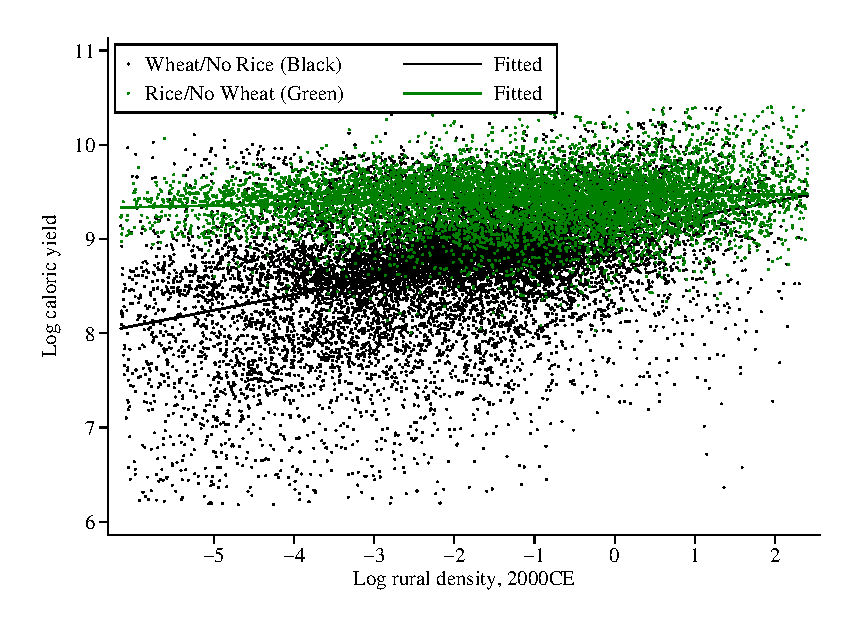
\includegraphics[width=1.0\textwidth]{fig_beta_crop.eps}
\end{center}
\vspace{-.5cm}\singlespacing {\footnotesize \textbf{Notes}: This figures shows the raw correlation of (log) caloric yield and (log) rural density for districts that are (a) suitable for wheat, but not for wet rice, and (b) suitable for wet rice but not for wheat. Rural population is from HYDE database \citep{hyde31}, and caloric yield is the author's calculations based on the data from \citet{galorozak2016}. The linear fits are from bivariate OLS regressions, without any fixed effects included. Based on equation (\ref{EQ_regress}), the slopes of these lines are estimates of $\beta$, the elasticity of agricultural output with respect to land.
}
\end{figure}


//////////////////////////////////////
// Create residual plot of baseline results
//////////////////////////////////////

qui reg ln_csi_yield urb_perc_2000 ln_light_mean i.state_id if dry_suit>0 & wet_suit==0, cluster(state_id)
predict csi_res_dry, res
qui reg ln_rurd_2000 urb_perc_2000 ln_light_mean i.state_id if dry_suit>0 & wet_suit==0, cluster(state_id)
predict rurd_res_dry, res

qui reg ln_csi_yield urb_perc_2000 ln_light_mean i.state_id if dry_suit==0 & wet_suit>0, cluster(state_id)
predict csi_res_wet, res
qui reg ln_rurd_2000 urb_perc_2000 ln_light_mean i.state_id if dry_suit==0 & wet_suit>0, cluster(state_id)
predict rurd_res_wet, res


scatter csi_res_dry rurd_res_dry if dry_suit>0 & wet_suit==0 & ln_csi_yield>0, msymbol(p) mcolor(black) ///
	|| lfit csi_res_dry rurd_res_dry if dry_suit>0 & wet_suit==0 & ln_csi_yield>0, clcolor(black) ///
	|| scatter csi_res_wet rurd_res_wet if dry_suit==0 & wet_suit>0, msymbol(p) mcolor(green) ///
	|| lfit csi_res_wet rurd_res_wet if dry_suit==0 & wet_suit>0, clcolor(green) ///
	xtitle("Residual log rural density, 2000CE") ytitle("Residual log caloric yield") ///
	ylabel(, angle(0) nogrid) graphregion(color(white)) /// xlabel(-5(1)2) ///
	legend(ring(0) pos(10) label(1 "Temperate (Black)") label(2 "Fitted") label(3 "Tropical (Green)") label(4 "Fitted"))
graph export "$output/fig_beta_crop.png", replace as(png)
graph export "$output/fig_beta_crop.eps", replace as(eps)

	


More broadly, HYDE's methodology of mapping of rural population may be driving our results. To assess this, we use a separate data source from the Global Rural-Urban Mapping Project (GRUMP), developed by \cite{Balketal2006}. This project also provides grid-cell level population counts, as well as ``urban masks'' that define cells within urban agglomerations. We extract the count of rural population in a given district from GRUMP as the count of population in all grid cells that are \textit{not} part of urban agglomerations. GRUMP's implicit rural population, then, will not necessarily conform to census reports of rural population (in principle, HYDE's count of rural population should conform). In the Appendix we show results using GRUMP's population data to measure rural density, and the results are consistent with the results from HYDE. There is one exception, which is that when we distinguish samples by their harvested area of crops, the estimated $\beta$ values are no longer statistically different between wheat and rice families. 

Combining this constraint with a positive relationship of living standards and population growth yields the canonical Malthusian model of stagnation \citep{ashraf2010dynamics}, and forms the basis for models of the transition from stagnation to sustained growth. The literature on the transition has grown large enough that it is difficult to provide a reasonable summary in a footnote. An overview of this unified growth literature can be found in \citet{Galor:2011uq}, who cites several key contributions \citep{gw00,galor2002natural,Hansen:2002fk,doepke2004accounting,cs2005,lagerlof2006,craftsmills2009,strulik2008population}. Explanations for the Great Divergence in income per capita are often framed in terms of these unified growth models \citep{kp2001,galor2008trading,vollrath2011,vv08,vv13,cs2015}. The Malthusian constraint features in quantitative work on contemporary developing countries that rely on agriculture \citep{Gollin:2007oq,Restuccia:2008hc,weilwilde2009,Gollin:2010ys,ev2016clim}, and is relevant for long-run growth in relatively rich countries due to possible limits to resources \citep{perettovalente2015}.